\section{Graph Matching}
\label{sec:graph-matching}

The graph matching problem is equivalent to Lawler's form of the quadratic assignment problem (QAP) from the combinatorial optimization literature.

Given two point sets the task is to establish $1:1$ correspondences between points in the respective sets.

\begin{definition}[Graph Matching]
Given $N_1,N_2 > 0$ and linear costs $c_{ij} \in \R$ for $(i,j) \in \R^{N_1 \times N_2}$ and quadratic costs $d \in \R^{N_1 \times N_2 \times N_1 \times N_2}$ the graph matching problem is
\begin{equation}
    \begin{array}{rl}
    \min\limits_{x \in \R^{N_1 \times N_2}} & \sum\limits_{ij \in E} c_{ij} x_{ij} + \sum_{ijkl \in T} d_{ijkl} x_{ij} x_{kl} \\ 
    \text{s.t.} 
    & \sum\limits_{j=1,\ldots,N_1} x_{ij} \leq 1 \quad \forall i\in [N_1] \\
    & \sum\limits_{i=1,\ldots,N_2} x_{ij} \leq 1 \quad \forall j\in [N_2] \\
    \end{array}
\end{equation}
\end{definition}

\begin{figure}[H]
    \begin{center}
        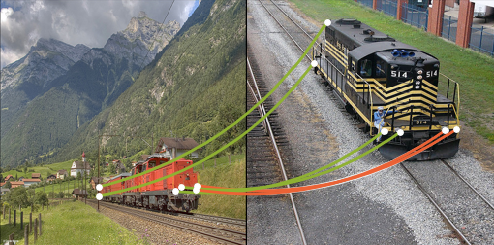
\includegraphics[width=\columnwidth]{images/train-matching.png}
        \caption{Keypoint matching in computer vision. Keypoints in both picturesgive rise to points sets for the graph matching problem.}
        \label{fig:cell-tracking}
    \end{center}
\end{figure}

\subsection{File Format}
\label{sec:graph-matching-file-format}

We use the file format introduced by~\cite{torresani2012dual}.

\begin{fileformat}
p (*$N_0$*) (*$N_1$*) A E 
a 1 (*$i_1$*) (*$j_1$*) (*$c_1$*)
.
.
.
a A (*$i_A$*) (*$j_A$*) (*$c_A$*)
e (*$a_1$*) (*$a'_1$*) (*$d_1$*)
.
.
.
e (*$a_E$*) (*$a'_E$*) (*$d_E$*)
\end{fileformat}
where $A$ is the number of linear assignment terms (those that are not listed are assumed to have value $\infty$) and $E$ is the number of pairwise terms (those that are not listed are assumed to have value $0$).
Linear assignments start with the identifier $a$ and are numbered from $1$ to $A$. They go from node $i_l$ to $j_l$ with cost $c_l$ for $l \in [A]$.
Quadratic costs start with the identifier $e$ and have cost $d_l$, $l \in [E]$.
The quadratic cost is incurred if both the $a_l$-th and $a'_l$-th assignments are active.

We also provide LP files for all instances.

\subsection{Benchmark datasets}

\subsubsection[Hotel \& House]{Hotel \& House\footnote{\url{https://keeper.mpdl.mpg.de/f/0fe3f173da55491cb10a/?dl=1
}}}
Matching of keypoints in two rigid objects~\cite{torresani2012dual}.
Images of the same object are taken at different angles and correspondences are computed from costs derived by appearance and geometric terms.
There are 105 instances for each object with $N_1 = N_2 = 30$ and dense linear and quadratic assignments.

%\subsubsection{Car \& Motor}
%Matching of keypoints in VOC PASCAL 2007 challenge pictures~\cite{everingham2010pascal} of cars and motorbikes. 
%Costs are generated as in~\cite{leordeanu2012unsupervised}.
%The \textcolor{red}{\#instances} instances contain up to 60 nodes and costs are dense.

%\subsubsection{Graph Flow}
%Tracking problems with large displacements~\cite{alhaija2015graphflow}. Keypoints in frames of RGB-D images are obtained by a Kinect camera are matched. The depth information provided by the Kinect camera is used for cost computation.

\subsubsection[Worms]{Worms\footnote{\url{https://keeper.mpdl.mpg.de/f/1058b4e0d8664c0bb0d5/?dl=1}}}
Matching nuclei of C.\ elegans for automatic annotation~\cite{kainmueller2014active} in bio-imaging. 
The 30 instances have up to $\max(N_1,N_2) = 1500$ points. Costs are sparse.


\subsection{Algorithms}
\begin{description}
\item[Semidefinite Programming~\cite{schellewald2005probabilistic}:] Semidefinite relaxation for graph matching.
\item[Dual Decomposition~\cite{torresani2012dual}:]
Subgradient ascent on a dual decomposition of graph matching into max-flow, linear assignment and enumeraive local subproblems.
\item[Hungarian BP~\cite{zhang2016pairwise}:]
Message passing using additionally a linear assignment solver.
\item[Message Passing~\cite{swoboda2017study}]
Several improved message passing schemes on different decompositions.
\item[Fusion Moves~\cite{hutschenreiter2021fusion}:] Explore subspaces of graph matchings generated randomly and solve with ILP solvers.
\item[Covering Trees~\cite{yarkony2010covering}:] Convert the graph matching problem to one large tree MRF with additional Lagrange multipliers and optimize with message passing.
\end{description}
